
\definecolor{myWhite}{HTML}{f7f7f7}
\definecolor{myGr1}{HTML}{c6c6c6}
\definecolor{myGr2}{HTML}{e3e3e3}
\definecolor{myCy}{HTML}{0396C1}
\pagestyle{empty}

\tikzset{
  emballage/.style={
    line width=0.6ex,
    rounded corners=6pt,
    draw= colorOne
  }
}

\newcommand{\briqueLait}{

  \begin{tikzpicture}[scale=0.4, every node/.style={scale=1.0}]

  %front
  \fill[myWhite,emballage] (4.3,-17.6) -- (-9.5,-14.25) -- (-9.5,8.2) -- (4.3,5.75) -- cycle;
  \path[decorate, decoration={text effects along path,
  text={Lait},
  text align=center,
  text effects/.cd,
  characters={text along path, scale=5,xslant=-.2},
  fit text to path
  }] (-8.8,-3.82) -- (3,-6.36);%MILK

  \coordinate (A) at (-7.1,-5.95);
  \coordinate (B) at (1.9,-8.02);

  \path[decorate, decoration={text effects along path,
  text={1L},
  text align={
    align=center,
    left indent=0.5,
    right indent=0.2%
  },
  text effects/.cd,
  characters={text along path, scale=3,xslant=-.2,text=cyan},
  fit text to path
  }] ($(A)!0.5!(B)$) -- ($(A)!1.0!(B)$);%package
  %upper
  \fill[myGr2 , emballage] (-1,10.6) -- (12.5,8.35) --  (4.3,5.75)  -- (-9.5,8.2) -- cycle;
  %lateral
  \fill[myGr1, emballage] (12.5,-14.25) -- (12.5,8.35) -- (4.3,5.75) -- (4.3,-17.6) -- cycle;
  %hole
  %\draw[fill=gray, emballage] (-6.1,8.6) .. controls (-6.5,8.5) and (-6.2,8.2) .. (-5.5,8.2) .. controls (-4.9,8.2) and (-4.4,8.4) .. (-4.8,8.6)-- cycle;
  %fold lateral 1
  \draw[emballage] (4.3,5.75)-- (8.1,1.2) -- (9,1.5) -- (9,2.7) -- (12.5,8.35);
  %fold lateral 2
  \fill[myGr1!90, emballage] (8,7) -- (8.1,1.2) -- (9,1.5) -- (9,2.7) -- (9.03,7.42) -- cycle;
  %fold upper
  \fill[myGr2!55, emballage]  (-4.46,9.79) -- (-5.42,9.43)-- (8,7) -- (9.03,7.42) -- cycle ;
  %straw
  %\shade[inner color=myCy!50,outer color=myCy, emballage] (-4.8,8.4) -- (-4.9,15.6) -- (-4.7,15.7) -- (-4.9,16) -- (-4.8,16.1) -- (-5,16.4) -- (-4.9,16.5) -- (-5.2,16.7) -- (-5.1,16.8) -- (-5.4,17) -- (-5.4,17.1) -- (-5.7,17.2) -- (-5.7,17.4) -- (-6,17.4) -- (-6.1,17.6) -- (-6.4,17.5) -- (-6.48,17.7) -- (-6.7,17.6) -- (-6.9,17.7) -- (-7.1,17.6) -- (-7.3,17.7) -- (-7.5,17.5) -- (-7.7,17.6) -- (-7.9,17.3) -- (-17.7,11.6) -- (-17.2,10.6) -- (-7.2,16.3) -- (-7.14,16.21) -- (-7.07,16.32)  -- (-6.98,16.24)  -- (-6.91,16.34)  -- (-6.85,16.3) -- (-6.79,16.35) -- (-6.72,16.27) -- (-6.64,16.33)  -- (-6.58,16.24)  -- (-6.5,16.28) -- (-6.48,16.2) -- (-6.4,16.2) -- (-6.4,16.1) -- (-6.3,16.1) -- (-6.31,16) -- (-6.18,16.01)-- (-6.23,15.89)-- (-6.13,15.85)-- (-6.21,15.76)-- (-6.06,15.73)-- (-6.13,15.64)-- (-6.05,15.56)-- (-6,8.4);
  \end{tikzpicture}

}

\tikzset{
    flechedimg/.style={
      <-,
      >=stealth,
      line width=3.8pt
    },
    flechedimd/.style={
      ->,
      >=stealth,
      line width=3.8pt
    },
    cote/.style={
      font=\small,
      inner sep=2pt
    }
  }

\newcommand{\briqueLaitScare}{

  \begin{tikzpicture}[scale=0.4, every node/.style={scale=1.0}]

  \coordinate (A) at (-9.5,8.2);
  \coordinate (B) at (4.3,5.75);
  \coordinate (C) at (-9.5,-14.25);
  \coordinate (D) at (12.5,8.35);

  \coordinate (AB) at ($(B)-(A)$);
  \coordinate (AC) at ($(C)-(A)$);
  \coordinate (BD) at ($(D)-(B)$);


  %front
  \fill[myWhite,emballage] (A) -- ($(A)!1.0!(B)$) -- ($(A)!1.0!(B) + 0.7*(AC)$) -- ($(A)!0.7!(C)$) -- cycle;
  %upper
  \fill[myGr2 , emballage] (A) -- (B) --  ($(B)!1.5!(D)$)  -- ($(A)+1.5*(BD)$) -- cycle;
  %lateral
  \fill[myGr1, emballage] (B) -- ($(B)!1.5!(D)$) -- ($($(B)!1.5!(D)$)+0.7*(AC)$ ) -- ($(B)+0.7*(AC)$) -- cycle;


  %dimension 

  \coordinate (AC07) at ($(A)!0.7!(C)$);

  \coordinate (AC07AB) at ($(AC07)+1.0*(AB)$);

  \coordinate (AC07ABBD) at ($(AC07AB)+1.5*(BD)$);

  \draw[]
      % Flèche A -> 20 % de AC07
      (A) edge[flechedimg, shift={($-0.2*(AB)$)}] ($(A)!0.2!(AC07)$)
      % Flèche C -> AC07, avec départ à 20 % de AC07-C
      ($(A)!0.8!(AC07)$) edge[flechedimd,shift={($-0.2*(AB)$)}] ($(A)!1.0!(AC07)$)

      % Dimension AB
      ($(AC07)!0.0!(AC07AB)$) edge[flechedimg,shift={($-0.4*(BD)$)}]  ($(AC07)!0.2!(AC07AB)$)
      ($(AC07)!0.8!(AC07AB)$) edge[flechedimd,shift={($-0.4*(BD)$)}]  ($(AC07)!1.0!(AC07AB)$)

      % % Dimension BD
      ($(AC07AB)!0.0!(AC07ABBD)$) edge[flechedimg,shift={($0.3*(AB)$)}]  ($(AC07AB)!0.2!(AC07ABBD)$)
      ($(AC07AB)!0.8!(AC07ABBD)$) edge[flechedimd,shift={($0.3*(AB)$)}]  ($(AC07AB)!1.0!(AC07ABBD)$)
    ;

  \path[
    decorate,
    decoration={
      text effects along path,
      text={10 cm},
      text align={
        align=center,
      },
      text effects/.cd,
      characters={
        text along path,
        scale=2,
        xslant=0.2,
        text=colorOne
      },
      fit text to path
    }
  ]
    ($(A)!0.7!(AC07) - 0.20*(AB)$)--($(A)!0.3!(AC07) - 0.20*(AB)$);

  \path[
    decorate,
    decoration={
      text effects along path,
      text={10 cm},
      text align={
        align=center,
      },
      text effects/.cd,
      characters={
        text along path,
        scale=2,
        xslant=1.2,
        text=colorOne
      },
      fit text to path
    }
  ]
    ($(AC07)!0.2!(AC07AB) - 0.5*(BD)$)--($(AC07)!0.8!(AC07AB) - 0.5*(BD)$);

  \path[
    decorate,
    decoration={
      text effects along path,
      text={10 cm},
      text align={
        align=center,
      },
      text effects/.cd,
      characters={
        text along path,
        scale=2,
        xslant=-1.2,
        text=colorOne
      },
      fit text to path
    }
  ]
    ($(AC07AB)!0.15!(AC07ABBD) + 0.4*(AB)$)--($(AC07AB)!0.85!(AC07ABBD) + 0.4*(AB)$);


  \path[decorate, decoration={text effects along path,
  text={Lait},
  text align=center,
  text effects/.cd,
  characters={text along path, scale=5,xslant=-.2},
  fit text to path,
  shift={(0.0,4.5)}
  }] (-8.8,-3.82) -- (3,-6.36);%MILK

  \coordinate (A) at (-7.1,-5.95);
  \coordinate (B) at (1.9,-8.02);

  \path[decorate, decoration={text effects along path,
  text={1L},
  text align={
    align=center,
    left indent=0.5,
    right indent=0.2%
  },
  text effects/.cd,
  characters={text along path, scale=3,xslant=-.2,text=cyan},
  fit text to path,
  shift={(0.0,6.5)}
  }] ($(A)!0.5!(B)$) -- ($(A)!1.0!(B)$);%package




  %\drawgrid{-10}{13}{-15}{10}{1}{1}

\end{tikzpicture}


}

\newcommand{\TikZapprox}{%
  \begin{tikzpicture}
      \node at (0,0) {$\approx $};
  \end{tikzpicture}
}



\newcommand{\imageCavendish}{%
    \begin{tikzpicture}
        % 1. L'image en arrière-plan (inner sep=0pt pour caler le repère exactement dessus)
        \node[inner sep=0pt] (img) at (0,0) {
            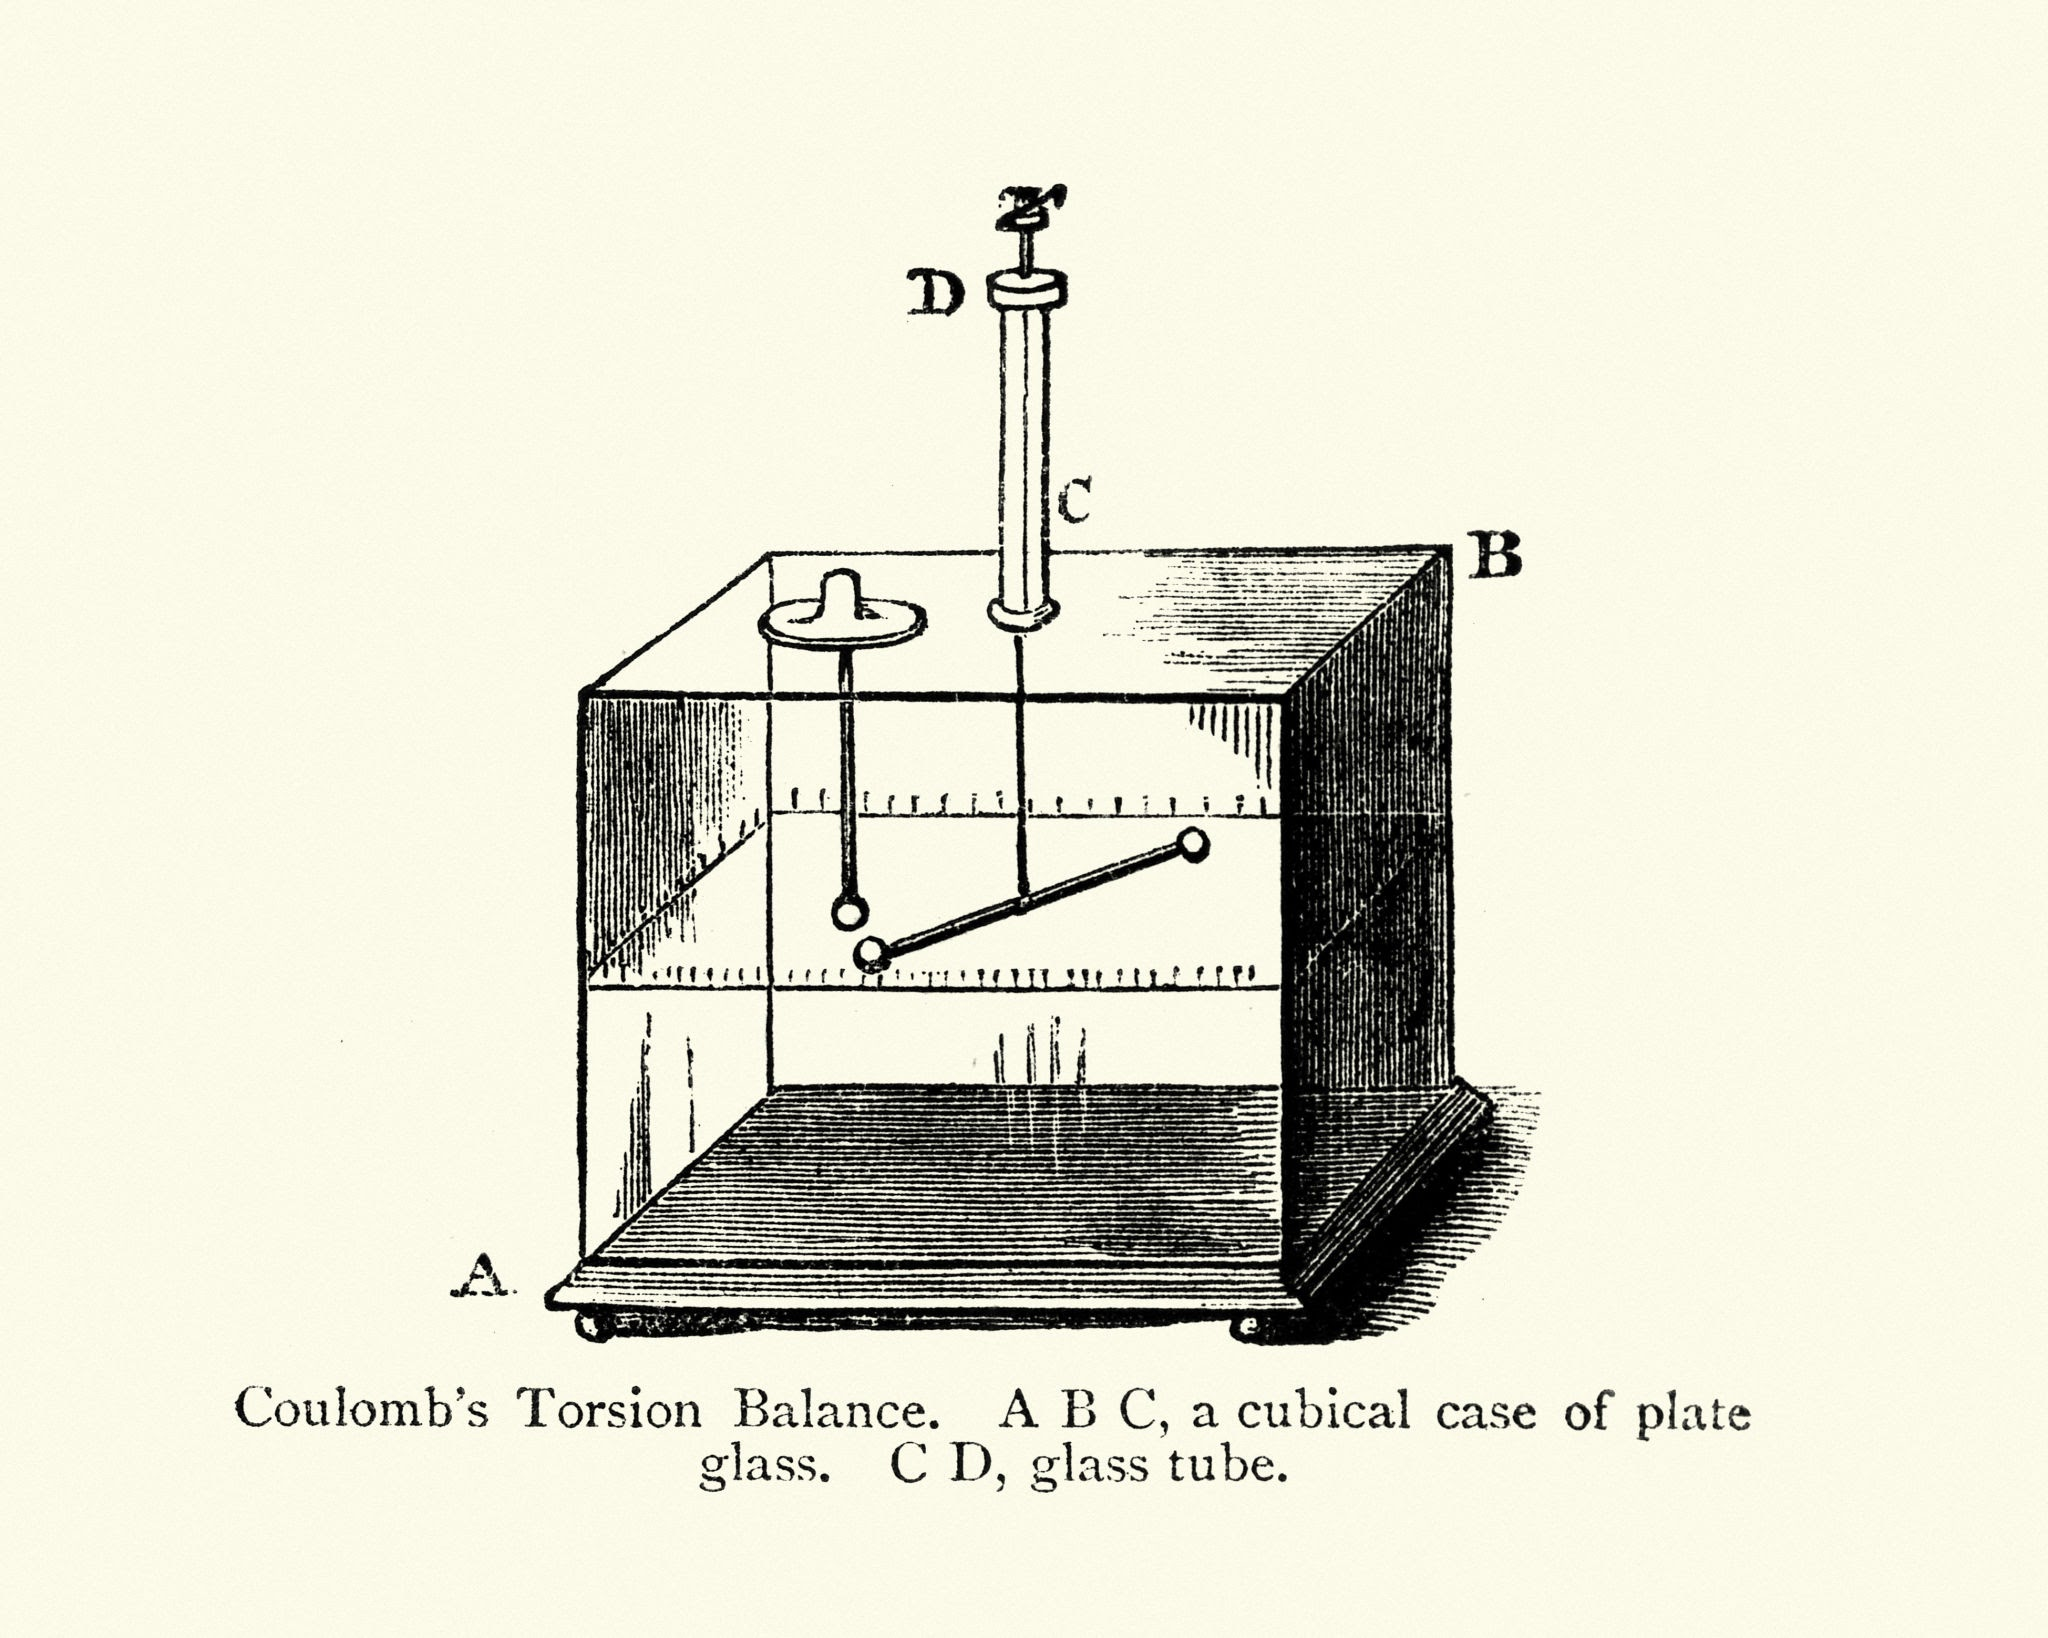
\includegraphics[trim={0.5cm 0.5cm 1.0cm 1.5cm}, clip, width=8cm]{./figures/tikz/imgs/cavendish_exp.jpeg}
        };

        % 2. Le repère dessiné par-dessus
        \begin{scope}[transform canvas={scale=0.5} , shift={(-6.0,1.0)}]
            \draw
                (-0.5,0)edge[->, line width=2.2pt, color=colorOne]node[pos=0.9, below, color=colorOne, font=\fontsize{20pt}{4}\bfseries\selectfont] {$\vec{e}_x$}(1.5,0) 
                (0,-0.5)edge[->, line width=2.2pt, color=colorOne]node[pos=0.9, left, color=colorOne, font=\fontsize{20pt}{4}\bfseries\selectfont] {$\vec{e}_z$}(0,1.5)
                (0.2,0.2)edge[->, line width=2.2pt, color=colorOne]node[pos=-1.3, color=colorOne, font=\fontsize{20pt}{4}\bfseries\selectfont] {$\vec{e}_y$}(-1,-1)
            ;
        \end{scope}
    \end{tikzpicture}%
}

% Macro pour la masse m' suspendue (sans tikzpicture imbriqué)
% Argument #1 : La coordonnée absolue de la masse (ex: D ou A-BD)
\newcommand{\MassePrime}[1]{%
    \begin{scope}[shift={(#1)}]
        \coordinate (OM) at (0,0);
        \coordinate (AM) at (0,-3);

        % Sphère m'
        \shade[line width=1.5pt, draw=colorOne, ball color=colorOne!20] (OM) circle [radius=0.5cm];
        \draw[line width=1.5pt, draw=colorOne, fill=colorOne!20] (OM) circle (0.05);

        % Fil support
        \draw[line width=1.0pt, color=colorOne] (OM) -- (AM);

        % Support hachuré
        \fill[
            fill=colorTwo, 
            pattern={Lines[
                angle=45,
                distance=3pt,
                line width=0.8pt
            ]},
            pattern color=colorThree 
        ] 
        ($(AM)-(1,0)$) -- ($(AM)+(1,0)$) -- ($(AM)+(1,-0.5)$) -- ($(AM)+(-1,-0.5)$) -- cycle;
        
        \draw[line width=1.0pt, color=colorOne] ($(AM)-(1,0)$) -- ($(AM)+(1,0)$);

        % Label m'
        \node at ($(OM)+(0,0.7)$) {$m'$};
    \end{scope}
}

\newcommand{\ShemaCavendishTroisD}{%
    \begin{tikzpicture}
        % 1. Définition des coordonnées absolues
        \coordinate (O) at (0,0);
        \coordinate (A) at (-4,-1);
        
        \coordinate (B) at (4,1);

        \def\vecOB{(B)-(O)}
        % Calcul propre de la coordonnée vectorielle OB
        \coordinate (vecOB) at ($(B)-(O)$);
        \coordinate (C) at (0,3);
        \coordinate (D) at (3,2);
        \coordinate (BD) at ($(D)-(B)$);
        \coordinate (A_prime) at ($(A)-(BD)$);

        % 2. Masses suspendues m' (OM placé exactement en D et A_prime)
        \MassePrime{D}
        \MassePrime{A_prime}

       

        % Masses m aux extrémités A et B
        \shade[line width=1.5pt, draw=colorOne, ball color=colorOne!20] (A) circle [radius=0.3cm];
        \shade[line width=1.5pt, draw=colorOne, ball color=colorOne!20] (B) circle [radius=0.3cm];

        % Points centraux
        \draw[line width=1.5pt, draw=colorOne, fill=colorOne!20] (O) circle (0.05);

         % 3. Tige centrale AB et masses m
        \draw[line width=2.5pt, color=colorOne] (A) -- (B);
        
        \draw[line width=1.5pt, draw=colorOne, fill=colorOne!20] (B) circle (0.05);
        \draw[line width=1.5pt, draw=colorOne, fill=colorOne!20] (A) circle (0.05);

        % Labels A, B, O, m
        \node at ($(A)!-0.1!(B)$) {$A$};
        \node at ($(A)!1.1!(B)$) {$B$};
        \node at ($(O)+(0,-0.5)$) {$O$};
        \node at ($(A)+(0,-0.7)$) {$m$};
        \node at ($(B)+(0,-0.7)$) {$m$};

        % 4. Fil de suspension principal et support haut (C)
        \draw[line width=1.5pt, color=colorOne] (O) -- (C);

        \fill[
            fill=colorTwo, 
            pattern={Lines[
                angle=45,
                distance=3pt,
                line width=0.8pt
            ]},
            pattern color=colorThree 
        ] 
        ($(C)-(1,0)$) -- ($(C)+(1,0)$) -- ($(C)+(1,0.5)$) -- ($(C)+(-1,0.5)$) -- cycle;

        \draw[line width=1.0pt, color=colorOne] ($(C)-(1,0)$) -- ($(C)+(1,0)$);

        % 5. Repère de coordonnées (axes e_x, e_y, e_z)
        \begin{scope}[shift={(-3.0,1.0)}, scale=0.5]
            \draw[->, line width=2.2pt, color=colorOne] ($(0,0) - 0.2*(4,0)$) -- ($(0,0) + 0.4*(4,0)$)  
                node[pos=1.2,  font=\fontsize{15pt}{4}\bfseries\selectfont] {$\vec{e}_x$};
            \draw[->, line width=2.2pt, color=colorOne] (0,-0.5) -- (0,1.5) 
                node[pos=1.2, font=\fontsize{15pt}{4}\bfseries\selectfont] {$\vec{e}_z$};
            \draw[->, line width=2.2pt, color=colorOne] ($(0,0) + 0.2*(4,1)$) -- ($(0,0) - 0.4*(4,1)$) 
                node[pos=1.2, font=\fontsize{15pt}{4}\bfseries\selectfont] {$\vec{e}_y$};
        \end{scope}

    \end{tikzpicture}%
}


\newcommand{\ShemaCavendishVertEqUn}{%
    \begin{tikzpicture}
        % 1. Définition des coordonnées absolues
        \coordinate (O) at (0,0);
        \coordinate (A) at (-4,0);
        
        \coordinate (B) at (4,0);

        \def\vecOB{(B)-(O)}
        % Calcul propre de la coordonnée vectorielle OB
        \coordinate (vecOB) at ($(B)-(O)$);
        \coordinate (C) at (0,3);
        \coordinate (D) at (4,4);
        \coordinate (BD) at ($(D)-(B)$);
        \coordinate (A_prime) at ($(A)-(BD)$);


        % Masses m aux extrémités A et B
        \shade[line width=1.5pt, draw=colorOne, ball color=colorOne!20] (A) circle [radius=0.3cm];
        \shade[line width=1.5pt, draw=colorOne, ball color=colorOne!20] (B) circle [radius=0.3cm];

        %\shade[line width=1.5pt, draw=colorOne, ball color=colorOne!20] (D) circle [radius=0.5cm];
        %\shade[line width=1.5pt, draw=colorOne, ball color=colorOne!20] (A_prime) circle [radius=0.5cm];

        % Points centraux
        \draw[line width=1.5pt, draw=colorOne, fill=colorOne!20] (O) circle (0.05);

         % 3. Tige centrale AB et masses m
        \draw[line width=2.5pt, color=colorOne] (A) -- (B);
        
        \draw[line width=1.5pt, draw=colorOne, fill=colorOne!20] (B) circle (0.05);
        \draw[line width=1.5pt, draw=colorOne, fill=colorOne!20] (A) circle (0.05);
        %\draw[line width=1.5pt, draw=colorOne, fill=colorOne!20] (D) circle (0.05);
        %\draw[line width=1.5pt, draw=colorOne, fill=colorOne!20] (A_prime) circle (0.05);

        \draw[dotted, line width=1.0pt, draw=colorOne!50] (O) circle (4.0);

        % Labels A, B, O, m
        \node at ($(A)!-0.1!(B)$) {$A$};
        \node at ($(A)!1.1!(B)$) {$B$};
        \node at ($(O)+(0,-0.3)$) {$O$};
        \node at ($(A)+(0,+0.7)$) {$m$};
        \node at ($(B)+(0,-0.7)$) {$m$};
        %\node at ($(D)+(0,+0.7)$) {$m'$};
        %\node at ($(A_prime)+(0,-0.7)$) {$m'$};


        % 5. Repère de coordonnées (axes e_x, e_y, e_z)
        \begin{scope}[shift={(0.0,3.0)}, scale=0.5]
            \draw[->, line width=2.2pt, color=colorOne] ($(0,0) - 0.0*(4,0)$) -- ($(0,0) + 0.4*(4,0)$)  
                node[pos=1.4,  font=\fontsize{15pt}{4}\bfseries\selectfont] {$\vec{e}_x$};
            \draw[->, line width=2.2pt, color=colorOne] (0,0.0) -- (0,-1.5) 
                node[pos=1.4, font=\fontsize{15pt}{4}\bfseries\selectfont] {$\vec{e}_y$};
            \draw[line width=2.2pt, color=colorOne] (0,0) circle (0.5); 
            
            \begin{scope}[]
                \clip (0,0) circle (0.5);
                \draw[line width=1.5pt, draw=colorOne, fill=colorOne!20] (0,0) circle (0.05);
                % \draw[line width=2.2pt, color=colorOne] 
                %     (-1,-1) -- (1,1) 
                %     (1,-1) -- (-1,1);
            \end{scope}

            \node[font=\fontsize{15pt}{4}\bfseries\selectfont , above=0.3cm ] at (0,0.0)  {$\vec{e}_z$};
        \end{scope}

    \end{tikzpicture}%
}


\newcommand{\ShemaCavendishVertEqDeux}{%
    \begin{tikzpicture}
        % 1. Définition des coordonnées absolues
        \coordinate (O) at (0,0);
        \coordinate (A) at (-4,0);
        \def\TheTa{30}
        \coordinate (A_deux) at ({-4*cos(\TheTa)}, {-4*sin(\TheTa)});
        
        \coordinate (B) at (4,0);
        \coordinate (B_deux) at ({4*cos(\TheTa)}, {4*sin(\TheTa)});

        \def\vecOB{(B)-(O)}
        % Calcul propre de la coordonnée vectorielle OB
        \coordinate (vecOB) at ($(B)-(O)$);
        \coordinate (C) at (0,3);
        \coordinate (D) at (4,4);
        \coordinate (BD) at ($(D)-(B)$);
        \coordinate (A_prime) at ($(A)-(BD)$);


        % Masses m aux extrémités A et B

        \shade[line width=1.5pt, draw=colorOne!50, ball color=colorOne!20] (A_deux) circle [radius=0.3cm];
        \shade[line width=1.5pt, draw=colorOne!50, ball color=colorOne!20] (B_deux) circle [radius=0.3cm];

        \shade[line width=1.5pt, draw=colorOne, ball color=colorOne!20] (D) circle [radius=0.5cm];
        \shade[line width=1.5pt, draw=colorOne, ball color=colorOne!20] (A_prime) circle [radius=0.5cm];

        % Points centraux
        \draw[line width=1.5pt, draw=colorOne, fill=colorOne!20] (O) circle (0.05);

        % 3. Tige centrale AB et masses m
        \draw[dashed, line width=2.5pt, color=colorOne!50] (A) -- (B);
        \draw[color=colorOne, line width=1.2pt] 
            (0,0) -- 
            (1,0) arc (0:\TheTa:1cm) 
            node[midway, right=2pt] {$\theta$}
            -- (0,0);
        \draw[line width=2.5pt, color=colorOne!50] (A_deux) -- (B_deux);

        \draw[->, color=colorThree, line width=1.5pt] 
            (0.5,0) arc (0:250:0.5cm) 
            node[midway, left=2pt] {$C$}
            ;

        \draw[] ($(A_deux)!0.1!(A_prime)$)edge[-> , >=Stealth , line width=2.5pt, color=colorOne!50]node[pos=0.5,right]{$\vec{F}$} ($(A_deux)!0.8!(A_prime)$);
        \draw[] ($(B_deux)!0.1!(D)$)edge[-> , >=Stealth , line width=2.5pt, color=colorOne!50]node[pos=0.5,right]{$\vec{F}$} ($(B_deux)!0.8!(D)$);
        
        %\draw[line width=1.5pt, draw=colorOne, fill=colorOne!20] (B) circle (0.05);
        %\draw[line width=1.5pt, draw=colorOne, fill=colorOne!20] (A) circle (0.05);
        \draw[line width=1.5pt, draw=colorOne, fill=colorOne!20] (D) circle (0.05);
        \draw[line width=1.5pt, draw=colorOne, fill=colorOne!20] (A_prime) circle (0.05);

        \draw[dotted, line width=1.0pt, draw=colorOne!50] (O) circle (4.0);

        % Labels A, B, O, m
        \node at ($(A_deux)!-0.1!(B_deux)$) {$A$};
        \node at ($(A_deux)!1.1!(B_deux)$) {$B$};
        \node at ($(O)+(0,-0.3)$) {$O$};
        \node at ($(A_deux)+(0,+0.7)$) {$m$};
        \node at ($(B_deux)+(0,-0.7)$) {$m$};
        \node at ($(D)+(0,+0.7)$) {$m'$};
        \node at ($(A_prime)+(0,-0.7)$) {$m'$};


        % 5. Repère de coordonnées (axes e_x, e_y, e_z)
        \begin{scope}[shift={(0.0,3.0)}, scale=0.5]
            \draw[->, line width=2.2pt, color=colorOne] ($(0,0) - 0.0*(4,0)$) -- ($(0,0) + 0.4*(4,0)$)  
                node[pos=1.4,  font=\fontsize{15pt}{4}\bfseries\selectfont] {$\vec{e}_x$};
            \draw[->, line width=2.2pt, color=colorOne] (0,0.0) -- (0,-1.5) 
                node[pos=1.4, font=\fontsize{15pt}{4}\bfseries\selectfont] {$\vec{e}_y$};
            \draw[line width=2.2pt, color=colorOne] (0,0) circle (0.5); 
            
            \begin{scope}[]
                \clip (0,0) circle (0.5);
                \draw[line width=1.5pt, draw=colorOne, fill=colorOne!20] (0,0) circle (0.05);
                % \draw[line width=2.2pt, color=colorOne] 
                %     (-1,-1) -- (1,1) 
                %     (1,-1) -- (-1,1);
            \end{scope}

            \node[font=\fontsize{15pt}{4}\bfseries\selectfont , above=0.3cm ] at (0,0.0)  {$\vec{e}_z$};
        \end{scope}

    \end{tikzpicture}%
}


\begin{tikzpicture}
  \clip[](-9, -2.3) rectangle (11, 2.5) ;
  \node[transform canvas={scale=0.8}] at (-6,0.) {
    \imageCavendish
  };
  \node[transform canvas={scale=0.4}] at (1,0) {\ShemaCavendishTroisD};
  \node[transform canvas={scale=0.4}] at (12,0) {\ShemaCavendishVertEqUn};
  \node[transform canvas={scale=0.4}] at (22,0) {\ShemaCavendishVertEqDeux};

  %\draw[line width=2.5ex , color = red ] (-9, -2.3) rectangle (11, 2.5) ;
  %\drawgrid{-9}{11}{-2.3}{2.5}{1}{1}
  
\end{tikzpicture}







